\subsection{Experimental Results}

We now evaluate the performance of our algorithm and hardware, including runtime comparison, power consumption measurements, and accuracy evaluation.

\paragraph{Runtime Results}

Figure~\ref{fig:latency-all} plots the runtime results of bilateral solver implementations on all our benchmarks, as a function of the spatial bandwidth.
Figure~\ref{fig:latency-all}a shows the runtime for the optimization portion of the solver, and Figure~\ref{fig:latency-all}b shows the runtime for the complete bilateral solver including pre-processing.

  % \begin{figure}[h!]
  %   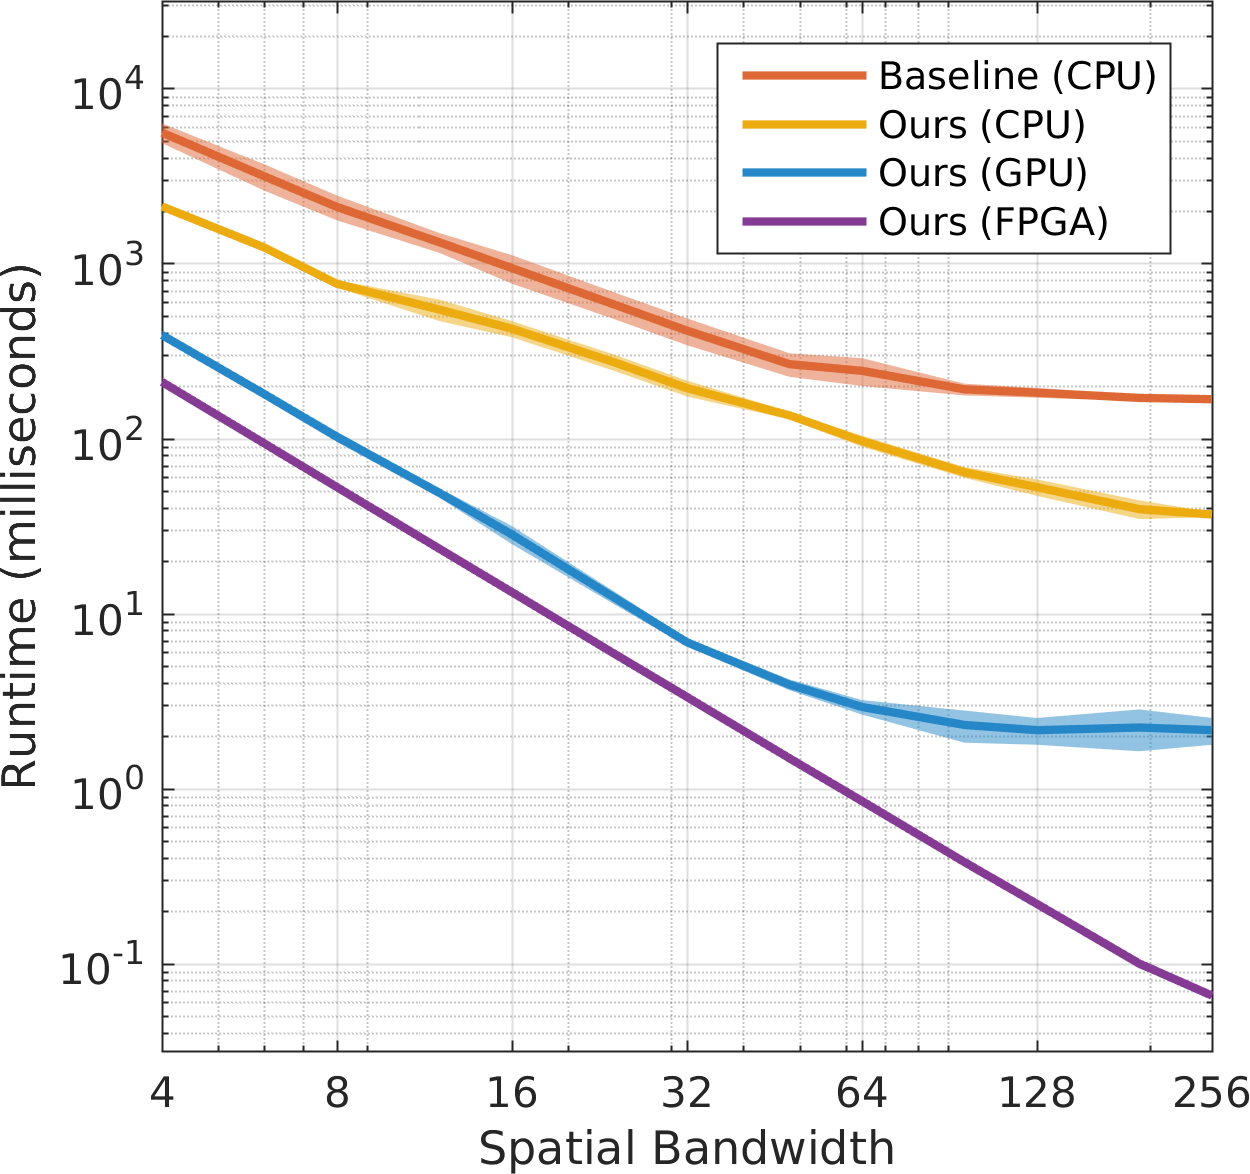
\includegraphics[width=0.235\textwidth]{hfbs-figs/runtime_opt.png}
  %   \caption{Runtime (Optimization Only)}
  % \end{figure}
  % \begin{figure}[h!]
  %   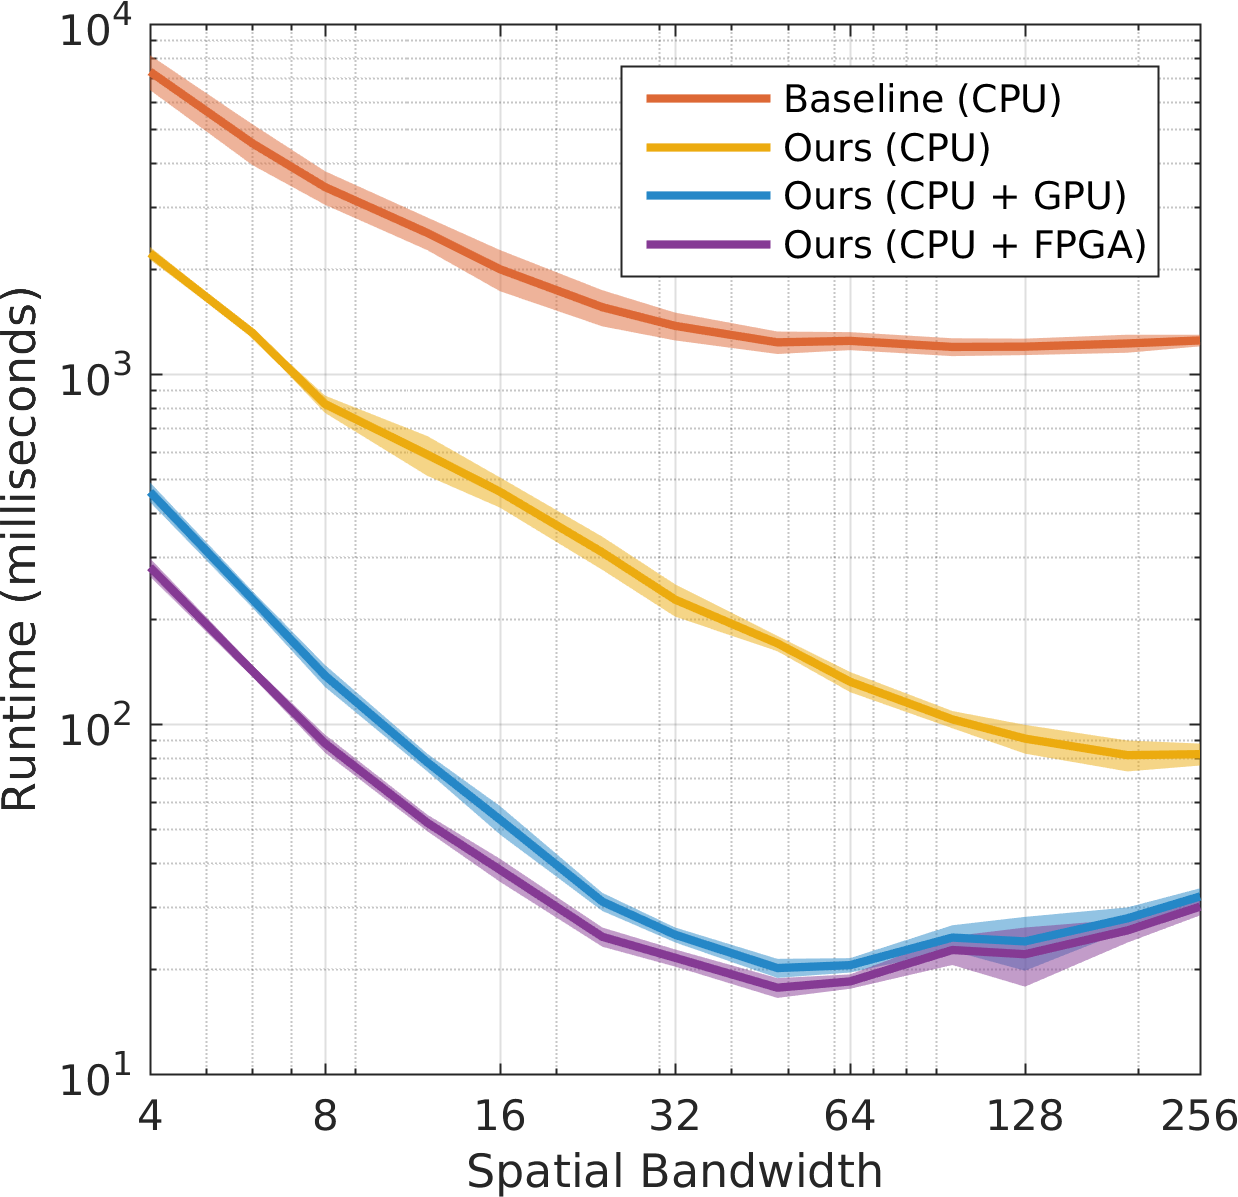
\includegraphics[width=0.235\textwidth]{hfbs-figs/runtime_total.png}
  %   \caption{Runtime (Total)}
  % \end{figure}
% \caption{Runtimes of the baseline, CPU, GPU, and FPGA implementations of HFBS, as a function of the spatial bandwidth ($\sigma_{xy}$ of Eq.~\ref{eq:hfbs-bilateral_affinity}).
% }

% \label{fig:latency-all}
% \end{figure}
\begin{figure}[!ht]
  \subfloat[Runtime (Optimization Only)]{%
    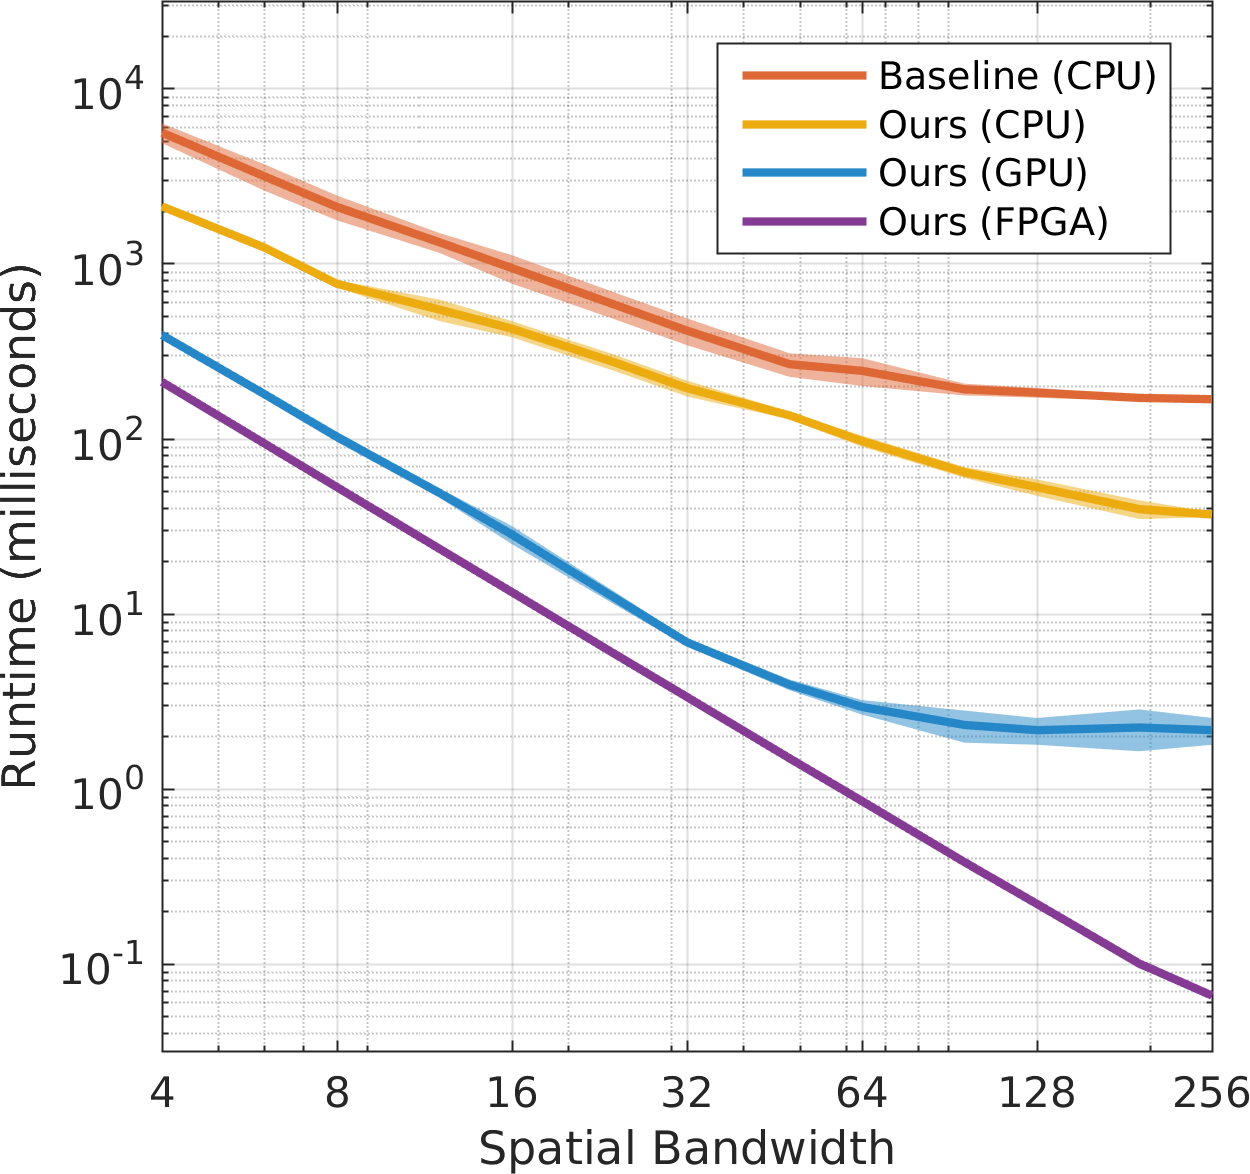
\includegraphics[width=0.45\textwidth]{hfbs-figs/runtime_opt.png}
    }
  \hfill
  \subfloat[Runtime (Total)]{%
    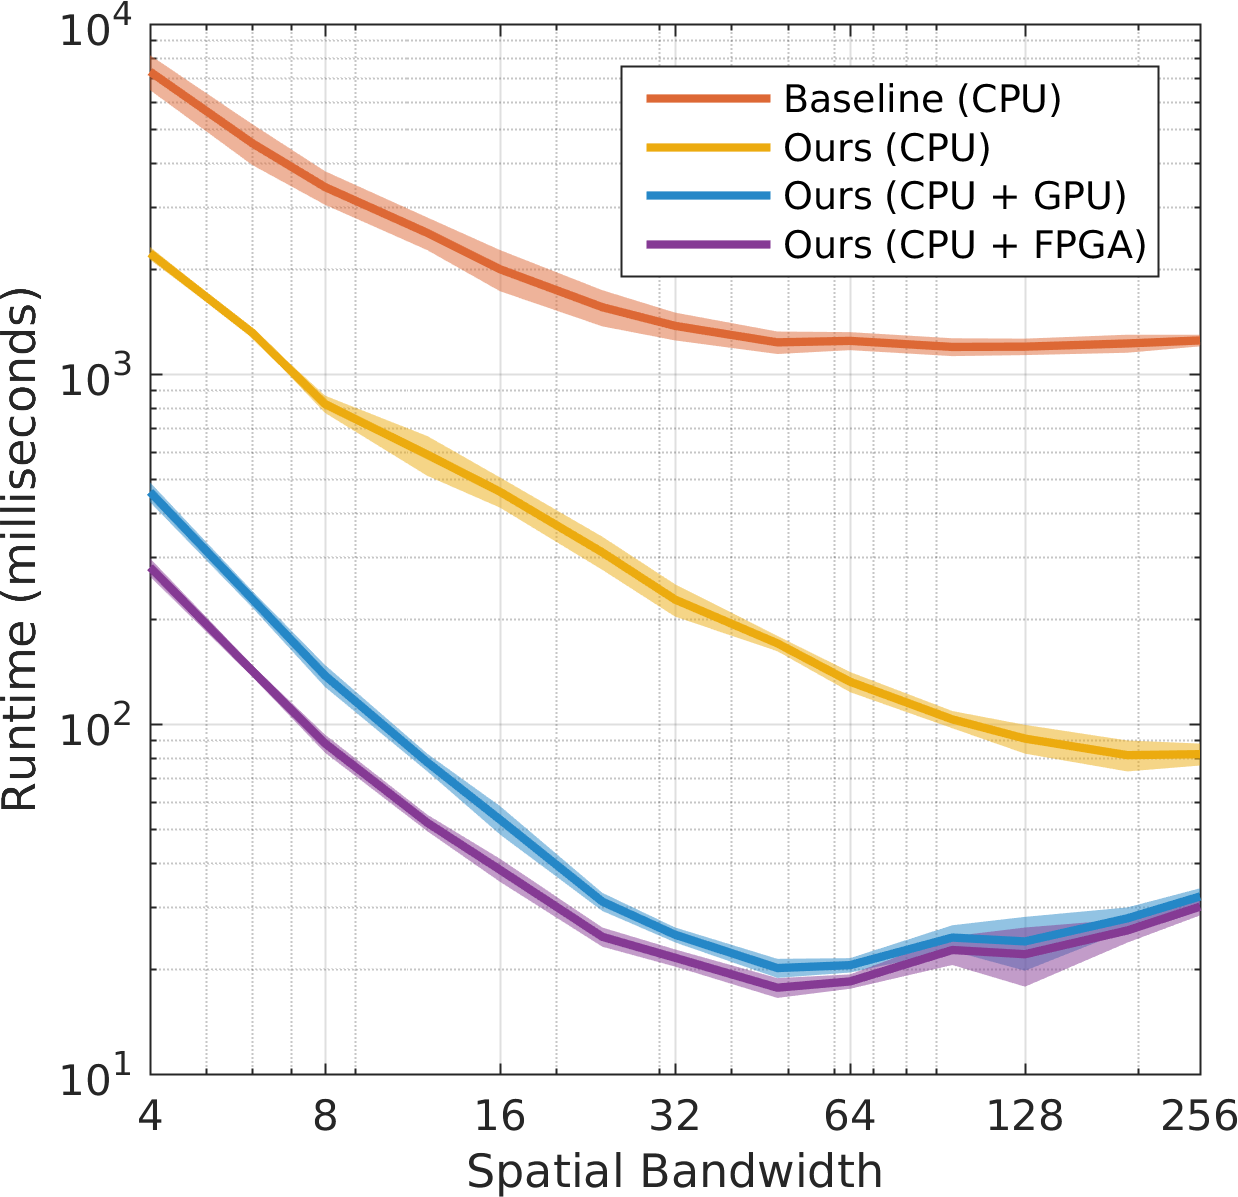
\includegraphics[width=0.45\textwidth]{hfbs-figs/runtime_total.png}
  }
  \caption{Runtimes of the baseline, CPU, GPU, and FPGA implementations of HFBS, as a function of the spatial bandwidth ($\sigma_{xy}$ of Eq.~\ref{eq:hfbs-bilateral_affinity}).}
  \label{fig:latency-all}
\end{figure}

As we increase the spatial bandwidth ($\sigma_{xy}$ of Eq.~\ref{eq:hfbs-bilateral_affinity}), we see that the overall grid size decreases, and runtimes shorten for all implementations.
We find that our algorithm outperforms the baseline on all platforms at all spatial bandwidths.
For optimization alone, CPU and FPGA results scale with the grid size, while the GPU results scales until the size of the grid is too small to fully utilize resources.
Because splatting and slicing is not accelerated on the FPGA, runtime for the entire bilateral solver does not scale as well at large grid sizes.

Table~\ref{table:jump_runtimes} highlights the runtime results specifically for the VR Video use-case, where $\sigma_{xy} = 12$ as in~\cite{googlejump}, as well as the power consumption of each hardware configuration. Our algorithm's speed outperforms the CPU baseline on all platforms evaluated, and our FPGA accelerator is significantly faster than the baseline while also reducing power consumption.

\begin{table}[h]
\centering
\caption{Runtimes for different variants of the bilateral solver on different hardware for the VR video use-case. Runtimes for optimization by itself and for the entire algorithm (problem construction/splatting, optimization, and slicing) are shown independently.}


\begin{tabular}{@{}lc@{}cc@{}cc}
\toprule
Algorithm / Platform & \multicolumn{2}{c}{Opt. (ms) } & \multicolumn{2}{c}{Total (ms)} & Power (W) \\ \midrule
 Baseline (CPU) & $1322$ & $\pm 171$ & $2529$ & $\pm 271$ & $16$ \\
                               Our Algorithm (CPU) & $545$ & $\pm 77$ & $588$ & $\pm 77$ & $152$ \\
                         Our Algorithm (CPU + GPU) & $49$ & $\pm 3$ & $78$ & $\pm 5$ & $245$ \\
                        Our Algorithm (CPU + FPGA) & $23$ & $\pm 1$ & $52$ & $\pm 3$ & $25$ \\
\bottomrule
\end{tabular}

\label{table:jump_runtimes}

\end{table}

Note that the CPU-only HFBS runtime reported in Table~\ref{table:jump_runtimes} is still far from the real-time requirement of 30 frames-per-second. The GPU and FPGA implementations get very close to real-time for $\sigma_{xy} = 12$, but still do not make it.
By selecting $\sigma_{xy} = 32$ and losing some accuracy, both FPGA and GPU implementations meet the real-time requirements.

We also observe that HFBS significantly reduces pre-processing. This is mainly caused by the elimination of the Jacobi preconditioner. The switch to a dense 3D bilateral grid improves available parallelism in the splat-slice routines as well.


\paragraph{Computation-communication Tradeoffs}

We consider the throughput of the data output as the ``communication cost'' for offloading, and the cost to compute the pipeline block as the ``computation cost''. We treat the communication cost as fixed for each block; it is simply the cost of offloading the data from each block, as shown in Figure~\ref{fig:vr-data-scale}.

\begin{figure}[h]
\centering
    \begin{center}
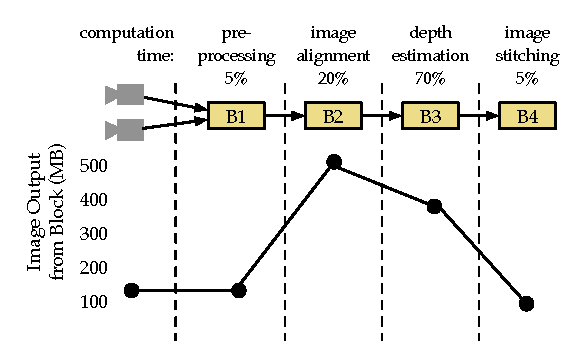
\includegraphics[width=.48\textwidth]{nsp-figs/vr_input_data.pdf}
    \end{center}
    \caption{Computation distribution and output data size for blocks in a VR video pipeline (2 of 16 cameras). }
    \label{fig:vr-data-scale}
\end{figure}

For all blocks except disparity refinement, we assume the computation cost to be the compute time evaluated using the ARM CPU baseline's performance numbers. We average the compute time for the disparity refinement block over five executions of the kernel over a frame. Because this processing flow can be pipelined across frames in a video stream, the ``total cost'' of the system can be considered to be dominated by the lowest-throughput block of the system.

Figure~\ref{fig:vr-fps} shows the runtime results of different pipeline configurations, uploaded on a networked connection to a viewing device supporting at least 30 FPS. We seek to uncover scenarios in which both computation and communication surpass our minimum frame rate of 30 FPS---if one or both costs falls below the threshold, the system cannot support real-time operation.

\begin{figure*}[h]
\centering
    \begin{center}
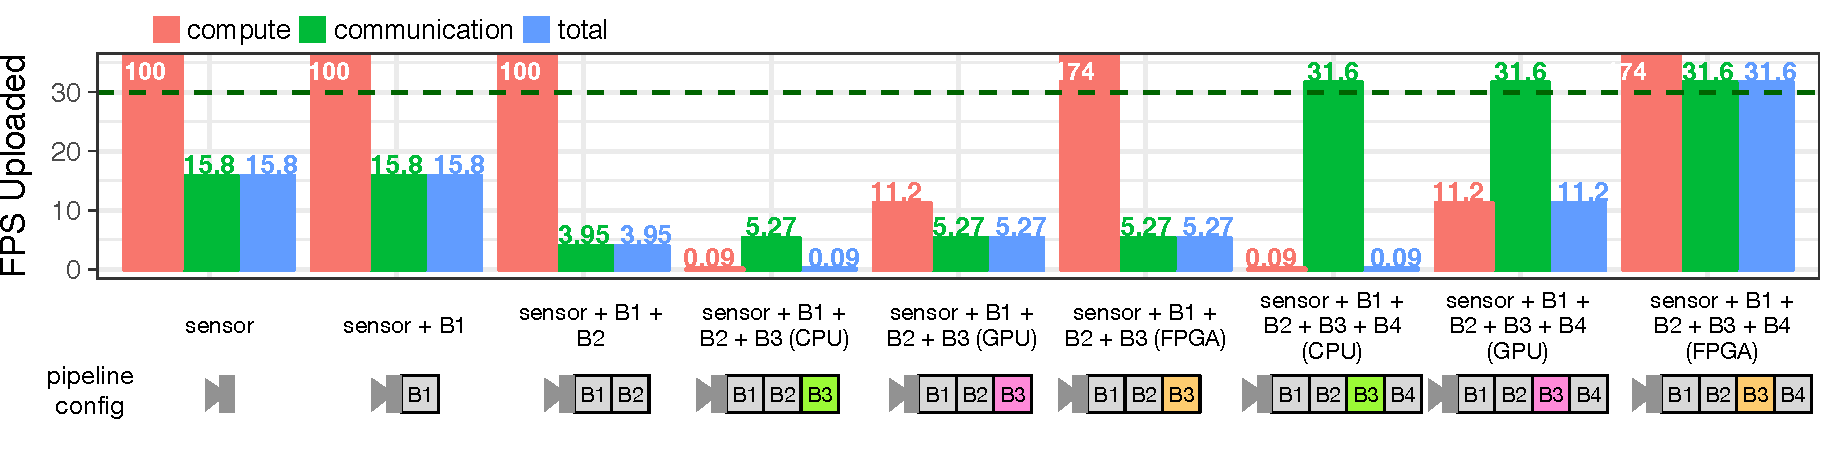
\includegraphics[width=1.0\textwidth]{nsp-figs/vr_compute_transfer.pdf}
    \end{center}
    \caption{Pipeline configurations with different bilateral smoothing implementations (CPU, GPU, FPGA), and resulting upload rates (frames per second). Only the full pipeline with FPGA acceleration can meet a 30 FPS upload requirement.}
    \label{fig:vr-fps}
\end{figure*}


For the first three scenarios, the cost of doing little computation before offloading is cheap, even on the ARM core, but the communication cost for the raw captured data falls short of our 30 FPS threshold. Computing the disparity refinement in $B_3$ is more costly, and the CPU and GPU implementations are not fast enough to support real-time operation. Moreover, the cost of offloading the computed depth maps before image stitching is significantly lower.

The computation cost of image stitching in $B_4$ is marginal compared to BSSA, as well, and the resulting FPS is virtually the same. The data size to communicate after $B_4$, however, is much smaller, as discussed in Figure~\ref{fig:vr-data-scale}, and is the only data size small enough to support real-time uploading. We find that the configuration with all the blocks processed in-camera and $B_3$ mapped to the FPGA is the only configuration where both computation and communication pass the threshold and support real-time processing.

Our analysis indicates that this camera system is primarily constrained by network bandwidth. For our evaluation, we assumed transfer speeds of 25 Gigabit Ethernet. As network connections grow faster, our results will trend towards offloading computation right off the sensor. For instance, at a hypothetical ultra-high-throughput network link of 400-Gb Ethernet, the 16-camera output can be uploaded at 395 FPS, reducing the efficiency incentive for in-camera processing in this scenario.

\paragraph{Depth Superresolution}
\label{sec:depth_superres}

Because our proposed model is an approximation to the bilateral solver, we
should expect some drop in the quality of our output relative to that
of \cite{BarronPoole2016}. To quantify this drop in accuracy, we evaluate on the
depth superresolution task of \cite{ferstl2013b}, which was the primary
evaluation used in \cite{BarronPoole2016}. We evaluate using the same experimental
setup and the same hyperparameters as \cite{BarronPoole2016} ($\sigma_{xy} = 8$, $\sigma_{l} = 4$), and report MSE with respect to ground truth from the Middlebury Stereo Dataset~\cite{middlebury-data}.

\begin{table}[h]
\centering
\caption{Depth Superresolution Task \cite{ferstl2013b}}

\begin{tabular}{@{}lcc@{}}
\toprule
Algorithm & Error (MSE) & Runtime (sec) \\
\midrule
            Chan \etal \cite{chan2008}   &  $ 3.89 $  &  $ 3.02 $   \\
            Min \etal  \cite{Min2014}   &  $ 3.78 $  &  $ 0.383 $  \\
    Domain Transform \cite{Gastal2011}   &  $ 3.60 $  &  $ 0.021 $  \\
           Ma \etal   \cite{Ma2013}   &  $ 3.53 $  &  $ 18 $  \\
        Zhang \etal  \cite{Zhang2014}   &  $ 3.51 $  &  $ 1.346 $  \\
    Guided Filter (Matlab) \cite{He2010}   &  $ 3.51 $  &  $ 0.434 $  \\
        Fast Guided Filter \cite{He2015}   &  $ 3.45 $  &  $ 0.225 $  \\
           Yang \etal  \cite{Yang2015}   &  $ 3.44 $  &  $ 0.304 $  \\
         Farbman \etal \cite{FFLS2008}   &  $ 3.24 $  &  $ 6.11 $  \\
          JBU \cite{Adams2010,Kopf2007}   &  $ 3.19 $  &  $ 1.98 $  \\
        Barron \& Poole \cite{BarronPoole2016}   &  $ 2.75 $  &  $ 0.234 $  \\ \hline
                               Our Model   &  $ 3.27 $  &   $ 0.047 \pm 0.002$ \\
\bottomrule
\end{tabular}

\label{table:depth_superres}
\end{table}

As can be seen in Table~\ref{table:depth_superres}, our model produces a slightly
higher error than that of \cite{BarronPoole2016}, but has a significantly
lower runtime (here we report runtime on a Nvidia 1080 Ti). This increase in error
is due to the fact that our model ignores color in the input image, and so has
difficulty distinguishing between pixels with different chroma but similar
luma. The images in this task are unusually colorful and ``cartoonish'',
by virtue of being a constructed vision task, so this increase in error
represents an upper-bound on the increased error we expect to see in natural scenes.
Even with this reduction in error, we see that
HFBS is significantly faster than all more-accurate techniques, and
significantly more accurate than all faster techniques.

% \begin{figure}[h]
% \centering
%   \subfloat[Input reference image,\\ from \cite{middlebury-data} ]{
%     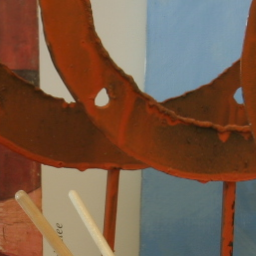
\includegraphics[width=0.235\textwidth]{hfbs-figs/super_depth/1_image.png}
%     }
%   \subfloat[Input noisy depth,\\ before filtering ]{
%     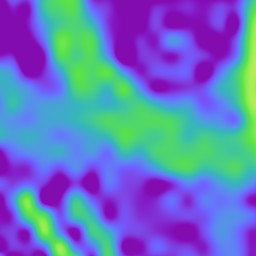
\includegraphics[width=0.235\textwidth]{hfbs-figs/super_depth/1_bicubic.png}
%     }
%   \subfloat[Improved depth \\ from \cite{BarronPoole2016} ]{
%     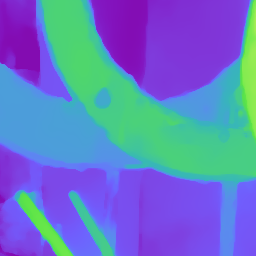
\includegraphics[width=0.235\textwidth]{hfbs-figs/super_depth/1_bsqs.png}
%     }
%   \subfloat[Our improved depth \\ (with HFBS) ]{
%     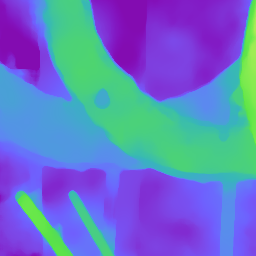
\includegraphics[width=0.235\textwidth]{hfbs-figs/super_depth/1_grayscale_bs.png}

\begin{figure}[!ht]
  \subfloat[Input reference image, from \cite{middlebury-data}]{%
    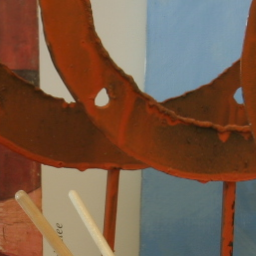
\includegraphics[width=0.45\textwidth]{hfbs-figs/super_depth/1_image.png}
  }
  \hfill
  \subfloat[Input noisy depth, before filtering]{%
    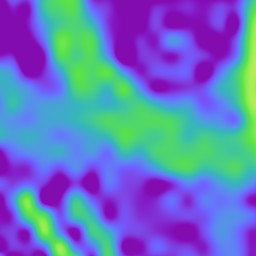
\includegraphics[width=0.45\textwidth]{hfbs-figs/super_depth/1_bicubic.png}
  }
  \subfloat[Improved depth from \cite{BarronPoole2016}]{%
    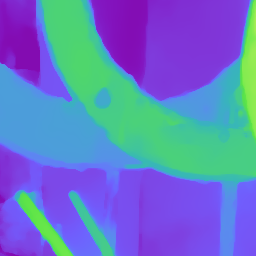
\includegraphics[width=0.45\textwidth]{hfbs-figs/super_depth/1_bsqs.png}
  }
  \hfill
  \subfloat[Our improved depth  (with HFBS)]{%
    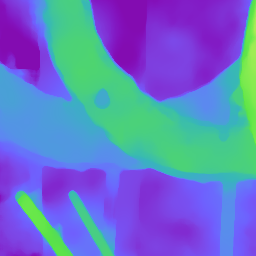
\includegraphics[width=0.45\textwidth]{hfbs-figs/super_depth/1_grayscale_bs.png}
  }
  \caption{A qualitative comparison of HFBS's performance
  compared to the model of \cite{BarronPoole2016} on the depth superresolution
  task of \cite{ferstl2013b}. HFBS produces similar output to \cite{BarronPoole2016} and is significantly faster.}
  \label{fig:depth_superres}
\end{figure}


We present qualitative results for this task in Figure~\ref{fig:depth_superres}.
As discussed in Section~\ref{sec:alg_mod}, HFBS requires double the iterations to achieve the same accuracy level of OBS, but still performs significantly faster.
We can see that our output depths are qualitatively very similar to those of
\cite{BarronPoole2016}, as expected.
